%<dscrpt>Fichier de déclarations Latex à inclure au début d'un élément de cours.</dscrpt>

\documentclass[a4paper]{article}
\usepackage[hmargin={1.8cm,1.8cm},vmargin={2.4cm,2.4cm},headheight=13.1pt]{geometry}

%includeheadfoot,scale=1.1,centering,hoffset=-0.5cm,
\usepackage[pdftex]{graphicx,color}
\usepackage[french]{babel}
%\selectlanguage{french}
\addto\captionsfrench{
  \def\contentsname{Plan}
}
\usepackage{fancyhdr}
\usepackage{floatflt}
\usepackage{amsmath}
\usepackage{amssymb}
\usepackage{amsthm}
\usepackage{stmaryrd}
%\usepackage{ucs}
\usepackage[utf8]{inputenc}
%\usepackage[latin1]{inputenc}
\usepackage[T1]{fontenc}


\usepackage{titletoc}
%\contentsmargin{2.55em}
\dottedcontents{section}[2.5em]{}{1.8em}{1pc}
\dottedcontents{subsection}[3.5em]{}{1.2em}{1pc}
\dottedcontents{subsubsection}[5em]{}{1em}{1pc}

\usepackage[pdftex,colorlinks={true},urlcolor={blue},pdfauthor={remy Nicolai},bookmarks={true}]{hyperref}
\usepackage{makeidx}

\usepackage{multicol}
\usepackage{multirow}
\usepackage{wrapfig}
\usepackage{array}
\usepackage{subfig}


%\usepackage{tikz}
%\usetikzlibrary{calc, shapes, backgrounds}
%pour la présentation du pseudo-code
% !!!!!!!!!!!!!!      le package n'est pas présent sur le serveur sous fedora 16 !!!!!!!!!!!!!!!!!!!!!!!!
%\usepackage[french,ruled,vlined]{algorithm2e}

%pr{\'e}sentation du compteur de niveau 2 dans les listes
\makeatletter
\renewcommand{\labelenumii}{\theenumii.}
\renewcommand{\thesection}{\Roman{section}.}
\renewcommand{\thesubsection}{\arabic{subsection}.}
\renewcommand{\thesubsubsection}{\arabic{subsubsection}.}
\makeatother


%dimension des pages, en-t{\^e}te et bas de page
%\pdfpagewidth=20cm
%\pdfpageheight=14cm
%   \setlength{\oddsidemargin}{-2cm}
%   \setlength{\voffset}{-1.5cm}
%   \setlength{\textheight}{12cm}
%   \setlength{\textwidth}{25.2cm}
   \columnsep=1cm
   \columnseprule=0.5pt

%En tete et pied de page
\pagestyle{fancy}
\lhead{MPSI-\'Eléments de cours}
\rhead{\today}
%\rhead{25/11/05}
\lfoot{\tiny{Cette création est mise à disposition selon le Contrat\\ Paternité-Pas d'utilisations commerciale-Partage des Conditions Initiales à l'Identique 2.0 France\\ disponible en ligne http://creativecommons.org/licenses/by-nc-sa/2.0/fr/
} }
\rfoot{\tiny{Rémy Nicolai \jobname}}


\newcommand{\baseurl}{http://back.maquisdoc.net/data/cours\_nicolair/}
\newcommand{\urlexo}{http://back.maquisdoc.net/data/exos_nicolair/}
\newcommand{\urlcours}{https://maquisdoc-math.fra1.digitaloceanspaces.com/}

\newcommand{\N}{\mathbb{N}}
\newcommand{\Z}{\mathbb{Z}}
\newcommand{\C}{\mathbb{C}}
\newcommand{\R}{\mathbb{R}}
\newcommand{\D}{\mathbb{D}}
\newcommand{\K}{\mathbf{K}}
\newcommand{\Q}{\mathbb{Q}}
\newcommand{\F}{\mathbf{F}}
\newcommand{\U}{\mathbb{U}}
\newcommand{\p}{\mathbb{P}}


\newcommand{\card}{\mathop{\mathrm{Card}}}
\newcommand{\Id}{\mathop{\mathrm{Id}}}
\newcommand{\Ker}{\mathop{\mathrm{Ker}}}
\newcommand{\Vect}{\mathop{\mathrm{Vect}}}
\newcommand{\cotg}{\mathop{\mathrm{cotan}}}
\newcommand{\sh}{\mathop{\mathrm{sh}}}
\newcommand{\ch}{\mathop{\mathrm{ch}}}
\newcommand{\argsh}{\mathop{\mathrm{argsh}}}
\newcommand{\argch}{\mathop{\mathrm{argch}}}
\newcommand{\tr}{\mathop{\mathrm{tr}}}
\newcommand{\rg}{\mathop{\mathrm{rg}}}
\newcommand{\rang}{\mathop{\mathrm{rg}}}
\newcommand{\Mat}{\mathop{\mathrm{Mat}}}
\newcommand{\MatB}[2]{\mathop{\mathrm{Mat}}_{\mathcal{#1}}\left( #2\right) }
\newcommand{\MatBB}[3]{\mathop{\mathrm{Mat}}_{\mathcal{#1} \mathcal{#2}}\left( #3\right) }
\renewcommand{\Re}{\mathop{\mathrm{Re}}}
\renewcommand{\Im}{\mathop{\mathrm{Im}}}
\renewcommand{\th}{\mathop{\mathrm{th}}}
\newcommand{\repere}{$(O,\overrightarrow{i},\overrightarrow{j},\overrightarrow{k})$}
\newcommand{\cov}{\mathop{\mathrm{Cov}}}

\newcommand{\absolue}[1]{\left| #1 \right|}
\newcommand{\fonc}[5]{#1 : \begin{cases}#2 \rightarrow #3 \\ #4 \mapsto #5 \end{cases}}
\newcommand{\depar}[2]{\dfrac{\partial #1}{\partial #2}}
\newcommand{\norme}[1]{\left\| #1 \right\|}
\newcommand{\se}{\geq}
\newcommand{\ie}{\leq}
\newcommand{\trans}{\mathstrut^t\!}
\newcommand{\val}{\mathop{\mathrm{val}}}
\newcommand{\grad}{\mathop{\overrightarrow{\mathrm{grad}}}}

\newtheorem*{thm}{Théorème}
\newtheorem{thmn}{Théorème}
\newtheorem*{prop}{Proposition}
\newtheorem{propn}{Proposition}
\newtheorem*{pa}{Présentation axiomatique}
\newtheorem*{propdef}{Proposition - Définition}
\newtheorem*{lem}{Lemme}
\newtheorem{lemn}{Lemme}

\theoremstyle{definition}
\newtheorem*{defi}{Définition}
\newtheorem*{nota}{Notation}
\newtheorem*{exple}{Exemple}
\newtheorem*{exples}{Exemples}


\newenvironment{demo}{\renewcommand{\proofname}{Preuve}\begin{proof}}{\end{proof}}
%\renewcommand{\proofname}{Preuve} doit etre après le begin{document} pour fonctionner

\theoremstyle{remark}
\newtheorem*{rem}{Remarque}
\newtheorem*{rems}{Remarques}

\renewcommand{\indexspace}{}
\renewenvironment{theindex}
  {\section*{Index} %\addcontentsline{toc}{section}{\protect\numberline{0.}{Index}}
   \begin{multicols}{2}
    \begin{itemize}}
  {\end{itemize} \end{multicols}}


%pour annuler les commandes beamer
\renewenvironment{frame}{}{}
\newcommand{\frametitle}[1]{}
\newcommand{\framesubtitle}[1]{}

\newcommand{\debutcours}[2]{
  \chead{#1}
  \begin{center}
     \begin{huge}\textbf{#1}\end{huge}
     \begin{Large}\begin{center}Rédaction incomplète. Version #2\end{center}\end{Large}
  \end{center}
  %\section*{Plan et Index}
  %\begin{frame}  commande beamer
  \tableofcontents
  %\end{frame}   commande beamer
  \printindex
}


\makeindex
\begin{document}
\noindent

\newcommand{\interFF}[2]{\left[ #1 , #2 \right] }
\newcommand{\interFO}[2]{\left[ #1 , #2 \right[ }
\newcommand{\interOF}[2]{\left] #1 , #2 \right] }
\newcommand{\interOO}[2]{\left] #1 , #2 \right[ }

\debutcours{Propriétés des fonctions dérivables}{beta 3.1 \tiny{ le \today}}

L'étude des \href{\baseurl C2063.pdf}{fonctions d'une variable réelle} est réparti entre divers documents.
\section{Dérivabilité. Calculs de dérivée}
\subsection{Fonction dérivable en un point.}
\begin{defi}
Soit $I$ un intervalle réel, $a\in I$ et $f$ une fonction de $I$ dans $\R$. On dit que $f$ est dérivable en $a$ si et seulement si il existe un réel $\lambda$ et une fonction $r$ définie dans $I$ tels que 
\begin{displaymath}
\forall x\in I,\; f(x) = f(a) + \lambda(x-a) + (x-a)r(x) \; \text{ avec } \; r\xrightarrow{a} 0
\end{displaymath}
\end{defi}\index{fonction dérivable en un point}\index{nombre dérivé en un point}
\begin{rems}
\begin{itemize}
  \item Pour une fonction $f$, il existe au plus un réel $\lambda$ vérifiant la propriété de définition. Pour une fonction dérivable en $a$, ce nombre est appelé \emph{nombre dérivé} en $a$. \newline 
  à justifier
  \item L'existence de la fonction $r$ n'est pas significative. On peut toujours définir par \og développement idiot\fg~ \index{développement idiot} une fonction $r$ vérifiant la relation
\begin{displaymath}
  r(x) = \frac{1}{x-a}\left( f(x) - f(a) - \lambda(x-a)\right) \text{ si } x\neq a \text{ et } r(a)=0
\end{displaymath}
Ce qui est significatif sa convergence en $a$ vers $0$.
\item Cette définition est un cas particulier de \emph{développement limité} d'ordre 1.\index{développement limité}
\end{itemize}
\end{rems}

\begin{prop}
  Soit $I$ un intervalle réel, $a\in I$ et $f$ une fonction de $I$ dans $\R$. Si $f$ est dérivable en $a$ alors elle est continue en $a$.
\end{prop}
\begin{rem}
 Ne jamais utiliser cette remarque formulée de cette manière. En revanche vous pouvez utiliser sa contraposée: \og cette fonction n'est évidemment pas dérivable en $a$ car elle n'est même pas continue en $a$\fg.
\end{rem}
\begin{demo}
  à compléter
\end{demo}
\begin{defi}
 Une fonction définie dans un intervalle $I$ est dite \emph{dérivable} dans $I$ si et seulement si elle est dérivable en tous les $a\in I$. La fonction dérivée est la fonction de $I$ dans $\R$ qui associe à $a$ le nombre dérivé de la fonction en $a$.
\end{defi}
Notation usuelle. Si $f$ est dérivable dans $I$ sa fonction dérivée est notée $f'$.
\index{dérivabilité à gauche} \index{dérivabilité à droite} \index{dérivabilité sur un intervalle} \index{fonction dérivée}
\begin{defi}
  Dérivabilité à droite, à gauche, sur un intervalle. fonction dérivée \newline
  à compléter
\end{defi}


\subsection{Exemples. Dérivées usuelles}
Pour ces premiers exemples, on aurait pu utiliser les taux de variation, je choisis délibérément les développements limités qui sont d'une plus grande portée.
Premiers exemples : les fonctions puissances ($n \in \N$) sont dérivables dans $\R$ et l'inversion (définie et dérivable dans $\R^*$):
\begin{prop}
Les fonctions puissances entières sont dérivables dans $\R$, la fonction inverse est dérivable dans $\R^*$.
\begin{displaymath}
  \left( x\mapsto x\right)' = \left( a\mapsto 1\right),\hspace{0.5cm} \left( x\mapsto x^n\right)' = \left( a\mapsto ax^{n-1}\right),\hspace{0.5cm}
  \left( x\mapsto \frac{1}{x}\right)' = \left(a\mapsto -\frac{1}{a^2} \right)
\end{displaymath} 
\end{prop}

\begin{demo}
Pour les fonctions puissances.
\begin{align*}
  &x = a + 1(x-a) + (x-a)r(x)            &r = \left( x\mapsto 0\right) \\
  &x^n = \left( a+(x-a)\right)^n = a^n + na^{n-1}(x-a) + (x-a)r(x) &r = \binom{n}{2}a^{n-2}(x-a) + \binom{n}{3}a^{n-3}(x-a)^2 + \cdots 
\end{align*}
Pour la fonction inverse.\newline
La clé de cette preuve est la formule
\begin{displaymath}
  \forall t\neq 1,\hspace{0.5cm} 1+t = \frac{1-t^2}{1-t} \; \Rightarrow \; \frac{1}{1-t} = 1 + t + \frac{t^2}{1-t}
\end{displaymath}

  On démontre la dérivabilité en $a\neq0$.
\begin{displaymath}
  \frac{1}{x} = \frac{1}{a+(x-a)} = \frac{1}{a} \frac{1}{1-\frac{-x+a}{a}} 
  = \frac{1}{a}\left(1 + \frac{-x+a}{a} + \frac{(\frac{-x+a}{a})^2}{1-\frac{-x+a}{a}}\right) 
  = \frac{1}{a} -\frac{1}{a^2}(x-a) + \frac{(x-a)^2}{a^2x}
\end{displaymath}
La fonction $r$ vérifie donc $r(x) = \frac{x-a}{a^2x}$ pour $x\neq a$ (et $r(a)=0$) ce qui assure qu'elle converge vers $0$ en $a$.
\end{demo}

Les autres dérivées usuelles viennent de l'axiomatique de la fonction exponentielle complexe : exponentielle réelle,  $\sin$, $\cos$ d'abord. Les autres fonctions dont on doit connaitre les dérivées sont obtenues à partir des précédentes avec des opérations y compris avec des considérations de bijection réciproque.

\subsection{Interprétation géométrique}
\begin{figure}[h]
 \centering
 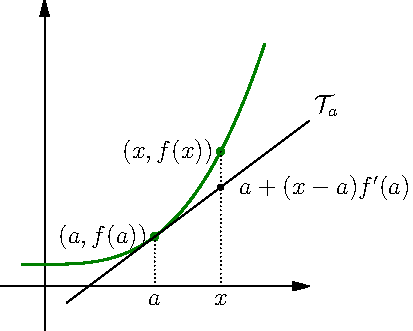
\includegraphics{./C2070_1.pdf}
 % C2070_1.pdf: 0x0 pixel, 0dpi, 0.00x0.00 cm, bb=
 \caption{Tangente au graphe d'une fonction}
 \label{fig:C2070_1}
\end{figure}

\begin{defi}[taux d'accroissement]\index{taux d'accroissement}
  Soit $I$ un intervalle réel, $a\in I$ et $f$ une fonction de $I$ dans $\R$. On appelle taux d'accroissement en $a$ de $f$, la fonction $\tau_{a}$ définie dans $I\setminus\left\lbrace a\right\rbrace$ par:
\begin{displaymath}
  \forall x \in I\setminus\left\lbrace a\right\rbrace,\; \tau_a(x) = \frac{f(x) - f(a)}{x - a}
\end{displaymath}
\end{defi}
\begin{rem}
 Le nombre $\tau_a(x)$ est la pente de la droite passant par les points $(a,f(a))$ et $(x,f(x))$ du graphe.
\end{rem}

\begin{prop}
Soit $I$ un intervalle réel, $a\in I$ et $f$ une fonction de $I$ dans $\R$. On dit que $f$ est dérivable en $a$ de nombre dérivé $\lambda$ si et seulemet si
$\tau_a \xrightarrow{a} \lambda$.
\end{prop}
\begin{demo}
  Rappellons que la fonction $r$ dont la convergence vers $0$ caractérise la dérivabilité en $a$ est définie par 
\[
 r(x) = 
\left\lbrace 
\begin{aligned}
 &\frac{f(x) -f(a) -\lambda(x-a)}{x-a} &\text{ si } x\neq a\\ &0 &\text{ si } x = a
\end{aligned}
\right. 
\]
On peut donc écrire
\[
 \forall x\neq a,\hspace{0.5cm} \tau_a(x) - \lambda = r(x). 
\]
La convergence de $\tau_a$ vers $\lambda$ est donc équivalente à celle de $r$ vers $0$.
\end{demo}

\begin{defi}\index{tangente au graphe et dérivabilité}
  Si $f$ est une fonction dérivable en $a$ de nombre dérivé $\lambda$ en $a$, la tangente au graphe au point de coordonnées $(a,f(a))$ est la droite (notée $\mathcal{T}_a$ sur la figure \ref{fig:C2070_1}) d'équation
\begin{displaymath}
  y - f(a) = \lambda (x-a)
\end{displaymath}
\end{defi}


\index{dérivabilité d'une réciproque}\index{tangente au graphe d'une réciproque}
\begin{prop}[dérivabilité d'une bijection réciproque]
 Soit $f$ une application bijective et continue d'un intervalle $I$ vers un intervalle $J$. Soit $a\in I$ et $b=f(a)\in J$. On suppose $f$ dérivable en $a$ de nombre dérivée $\lambda$ non nul. Alors $f^{-1}$ est dérivable en $b$ de nombre dérivé $\frac{1}{\lambda}$.\newline
 Les tangentes en $(b,a)$ au graphe de $f^{-1}$ et en $(a,b)$ au graphe de $f$ sont symétriques par rapport à la première bissectrice (figure \ref{fig:C2070_2}).
\end{prop}
\begin{figure}[h]
 \centering
 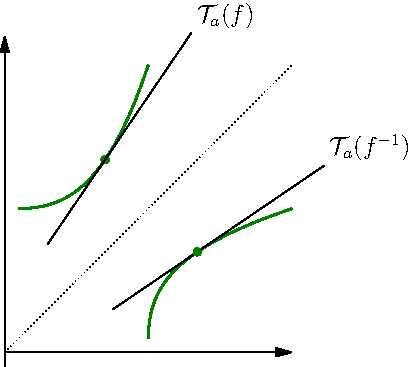
\includegraphics{./C2070_2.pdf}
 \caption{Tangente d'une bijection réciproque}
 \label{fig:C2070_2}
\end{figure}

\begin{demo}
Notons $g=f^{-1}$. D'après le théorème de la continuité d'une bijection réciproque, on sait que $g$ est continue dans $J$ en particulier en $b$. La dérivabilité de $f$ en $a$ se traduit par l'existence d'une fonction $r$ définie dans $I$ et qui converge vers $0$ en $a$ telle que
\[
\forall x \in I, \; f(x) = f(a) + \lambda(x-a) + (x-a)r(x) 
\]
Notons $\tau_f$ le taux d'accroissement de $f$ en $a$ (définie dans $I\setminus\{a\}$) et $\tau_g$ celui de $g$ en $b$ (définie dans $J\setminus\{b\}$). On sait que
\[
 f \text{ dérivable en } a \Leftrightarrow r\xrightarrow{a} 0 \Leftrightarrow \tau_f \xrightarrow{a} \lambda.
\]
D'autre part,
\[
 \forall y \in J\setminus\{b\},\;
 \tau_g(y) = \frac{g(y) - g(b)}{y-b}
 =\frac{1}{\frac{f(x) - f(a)}{x - a}}
\]
en posant $x=g(y)$. On en déduit 
\[
 \tau_g = \frac{1}{\tau_f \circ g} \Rightarrow \tau_g \xrightarrow{b} \frac{}{\lambda}
\]
d'après la dérivabilité de $f$, la continuité de $f$ et la composition des fonctions admettant une limite finie.\newline
Notons $\mathcal{T}_a(f)$ et $\mathcal{T}_b(f^{-1})$ respectivement la tangente en $(a,b)$ au graphe de $f$ et la tangente en $(b,a)$ au graphe de $f^{-1}$.
\[
 \forall (x,y) \in \R^2,\;
\left\lbrace 
\begin{aligned}
 (x,y) \in \mathcal{T}_a(f) \Leftrightarrow y &= a + \lambda(x-a) \\
 (x,y) \in \mathcal{T}_b(f^{-1}) \Leftrightarrow y &= b + \frac{1}{\lambda}(x-b) 
\end{aligned}
\right. 
\]
On peut transformer la deuxième équation:
\[
 (x,y) \in \mathcal{T}_b(f^{-1}) \Leftrightarrow \lambda(y - b) = x-b 
 \Leftrightarrow x = b +\lambda(y-x) 
 \Leftrightarrow (y,x) \in \mathcal{T}_a(f).
\]
Ceci montre la symétrie des deux tangentes.
\end{demo}

\subsection{Opérations - Composition}
\begin{prop}
 Soit $f$ et $g$ deux fonctions définies dans un intervalle $I$ et dérivable en $a\in I$ avec respectivement $\lambda_f$ et $\lambda_g$ comme nombre dérivé. Les fonctions $f+g$ et $fg$ sont alors dérivables en $a$ avec :
\begin{displaymath}
 \text{ nb dérivé de $f+g$ en $a$ } = \lambda_f + \lambda_g, \hspace{1cm} \text{ nb dérivé de $fg$ en $a$ } = \lambda_f g(a) + f(a) \lambda_g
\end{displaymath}
\end{prop}
\begin{demo}
 à compléter
Il s'agit d'effectuer les opérations sur les développements limités en \emph{rangeant directement} les termes par ordre décroissant.\newline
Le développement du produit comprend 9 termes groupés en paquets de 1 (ordre 0), 2 (ordre 1), 6 (ordre 2). Le paquet des 6 derniers termes se met sous la forme $(x-a)\rho(x)$.
\begin{multline*}
\left. 
\begin{aligned}
f(x) &= f(a) + \lambda_f(x-a) + (x-a)r_f(x) \\
g(x) &= g(a) + \lambda_g(x-a) + (x-a)r_g(x) 
\end{aligned}
\right\rbrace \Rightarrow
f(x)g(x) = f(a)g(a) + \left( f(a)\lambda_g + \lambda_f g(a)\right)(x-a) +(x-a)\rho(x) \\
\text{ avec } \rho(x) = f(a)r_g(x) + g(a)r_f(x) + \lambda_f \lambda_g(x-a) + \lambda_f(x-a)r_g(x) + \lambda_g(x-a)r_f(x) + (x-a)r_f(x)r_g(x) . 
\end{multline*}
L'expression de $\rho$ montre que $\rho \xrightarrow{a} 0$ car $r_f$ et $r_g$ tendent vers $0$ en $a$.
\end{demo}

\begin{prop}
 Soit $f$ une fonction définie dans un intervalle $I$ et dérivable en $a\in I$. Soit $g$ une fonction définie dans un intervalle $J$ et dérivable en $b\in J$. Lorsque $f(I)\subset J$ et $b=f(a)$, la fonction $g\circ f$ est dérivable en $a$ avec :
\begin{displaymath}
 (g \circ f)'(a) = f'(a) g'(f(a))
\end{displaymath}
\end{prop}
\index{dérivabilité d'une  fonction composée}
\begin{demo}
 \'Ecrivons les définitions des dérivabilités : de $f$ en $a$ et de $g$ en $b$. Il existe des fonctions $\varepsilon_1$ et $\varepsilon_2$ qui convergent vers $0$ respectivement en $a$ et en $b$ telles que :
\begin{align*}
 \forall x\in I :\; f(x) &= b +(x-a)f'(a)+(x-a)\varepsilon_1(x)\\
 \forall y\in J :\; g(y) &= g(b) +(y-b)g'(b)+(y-b)\varepsilon_2(y)
\end{align*}
On en déduit :
\begin{multline*}
 g\circ f(x) = g\circ f(a) + (f(x)-b)g'(b) +(f(x)-b)\varepsilon_2(f(x)) \\
= g\circ f(a) + (x-a)f'(a)g'(b) +(x-a)\varepsilon_1(x)g'(b) + (f(x)-b)\varepsilon_2(f(x)) \\
= g\circ f(a) + (x-a)f'(a)g'(b) +
(x-a)\underset{\xrightarrow{a}0}{\underbrace{\left( \varepsilon_1(x)g'(b) + \frac{f(x)-b}{x-a}\varepsilon_2(f(x))\right)}} 
\end{multline*}
\end{demo}
\begin{rems}
 \begin{enumerate}
  \item On déduit de la proposition sur la dérivée d'une composée l'expression de la dérivée d'une puissance.
\begin{displaymath}
 f^\alpha = \exp \circ (\alpha \ln \circ f) \Rightarrow (f^\alpha)' = \alpha f' f^{\alpha -1}
\end{displaymath}
  \item Dérivée d'une bijection réciproque dérivable. Soit $f$ et $g$ deux bijections dérivables réciproques l'une de l'autre, respectivement de $I$ dans $J$ et de $J$ dans $I$. Pour tout $x$ de $I$ : $g\circ f(x)=x$ donc
\begin{displaymath}
 g'(f(x))f'(x)=1
\end{displaymath}
 Ceci montre que $f'$ et $g'$ ne s'annulent pas avec :
\begin{displaymath}
 \forall y\in J : g'(y)=\frac{1}{f'(g(y))}
\end{displaymath}
Il faut bien noter que \emph{ceci ne démontre pas la dérivabilité des fonctions}.
 \end{enumerate}
\end{rems}
\index{exemple de dérivée non continue}\label{derpascont}
\textbf{Exemple de fonction dérivable dans $\R$ dont la dérivée n'est pas continue en $0$.}
\begin{align*}
  \R &\rightarrow \R \\
  x  &\mapsto f(x)=
\left\lbrace 
 \begin{aligned}
&0 &\text{ si } x=0 \\
&x^2 \sin(\frac{1}{x^2}) & \text{ si } x\neq0 
 \end{aligned}
\right. 
\end{align*}
Elle est dérivable dans $\R$ de dérivée
\begin{displaymath}
 x\mapsto f'(x)=
\left\lbrace 
 \begin{aligned}
&0 &\text{ si } x=0 \\
&2x \sin(\frac{1}{x^2}) -\frac{2}{x}\cos(\frac{1}{x^2})& \text{ si } x\neq0 
 \end{aligned}
\right.
\end{displaymath}
La dérivabilité en $x\neq 0$ ainsi que l'expression de la dérivée résultent des théorèmes sur les opérations et la composition. En $0$, la définition de $f$ permet d'écrire un développement
\begin{displaymath}
 |\sin(\frac{1}{x^2})|\leq 1 \Rightarrow f(x) =o(x)= f(0)+0(x-0)+o(x-0)
\end{displaymath}
ce qui est la définition même de $f$ dérivable en $0$ avec $f'(0)=0$.


\subsection{Dérivées successives}
Notations $f''$, $f^{(2)}$, $f^{(n)}$, classes $\mathcal{D}^n(I)$, $\mathcal{C}^n(I)$, $\mathcal{C}^{\infty}(I)$.
\begin{displaymath}
  \mathcal{C}^0(I) \supset \mathcal{D}^1(I) \supset \mathcal{C}^1(I) \supset \cdots
  \supset \mathcal{C}^n(I) \supset \mathcal{D}^{n+1}(I) \supset \mathcal{C}^{n+1}(I) \supset \cdots \supset \mathcal{C}^{\infty}(I)
\end{displaymath}

\index{formule de Leibniz}
\begin{prop}[formule de Leibniz]
 Soient $f$ et $g$ deux fonctions $n$ fois dérivables dans un intervalle $I$. La fonction $fg$ est alors $n$ fois dérivable avec :
\begin{displaymath}
 (fg)^{(n)}=\sum_{k=0}^n\binom{n}{k}f^{(k)}g^{(n-k)}
\end{displaymath}
\end{prop}
\begin{demo}
 La démonstration est analogue à celle de la formule du binôme (voir \href{\baseurl C2003.pdf}{Calculs usuels. Sommations}).
\end{demo}

\index{fonctions de classe $\mathcal C^k$}
\section{Théorème de Rolle}
\subsection{Dérivée et extremum local}
\index{extrémum local}\index{extrémum global}\index{minimum local}\index{minimum global}\index{maximum local}\index{maximum global}
\begin{defi}
Pour une fonction $f$ définie dans un intervalle $I$ et à valeurs réelles, on définit les notions de minimum local, minimum global, maximum local, maximum global, extrémum local, extrémum global.\newline
Il s'agit d'éléments de $I$. Précisons dans tableau la condition que doit vérifier $a\in I$ pour être un de ces objets
\begin{center}
\renewcommand{\arraystretch}{1.5}
\begin{tabular}{|l|c|}\hline
minimum global & $\forall x \in I, f(a) \leq f(x)$   \\ \hline
maximum global & $\forall x \in I, f(x) \leq f(a)$ \\ \hline 
minimum local  & $\exists \alpha >0 \text{ tq },\, \forall x \in \left] a-\alpha, a+\alpha\right[ , f(a) \leq f(x)$ \\ \hline 
maximum local  & $\exists \alpha >0 \text{ tq },\, \forall x \in \left] a-\alpha, a+\alpha\right[ , f(x) \leq f(a)$ \\ \hline
extrémum global & maximum ou minimum global \\ \hline
extrémum local & maximum ou minimum local \\ \hline
\end{tabular}
\end{center}

\end{defi}

\begin{prop}
 Soit $I$ un intervalle et $a$ un point de $I$ qui n'est pas une extrémité. Soit $f$ une fonction définie dans $I$. Si $a$ est un extrémum local de $f$ et si $f$ est dérivable en $a$ alors $f'(a)=0$.
\end{prop}
\begin{demo}
 Comme $a$ est un point intérieur à $I$ qui est un extremum local de $f$, il existe un $\alpha>0$ assez petit pour que $]a-\alpha, a+\alpha[$ soit inclus dans $I$ et que $f(x)-f(a)$ garde un signe constant dans cet intervalle (négatif ou nul si $a$ est un maximum, positif ou nul si $a$ est un minimum).\newline
Supposons par exemple que $a$ est un maximum. On peut passer à la limite dans les inégalités obtenues de chaque côté de $a$:
\begin{align*}
 &\forall x\in ]a-\alpha, a[: &f(x)-f(a)\leq 0, & x-a<0 &\frac{f(x)-f(a)}{x-a}\xrightarrow{a^{+}}f'(A)\Rightarrow f'(a)\geq 0 \\
&\forall x\in ]a, a+\alpha[: &f(x)-f(a)\leq 0, & x-a>0 &\frac{f(x)-f(a)}{x-a}\xrightarrow{a^{-}}f'(A)\Rightarrow f'(a)\leq 0  
\end{align*}
On obtient donc bien $f'(a)=0$. Lorsque $a$ est un minimum, le raisonnement est identique (les signes sont inversés). On peut aussi considérer $-f$.
\end{demo}
\begin{rems}
 \begin{itemize}
  \item La condition n'est pas suffisante. Par exemple soit $f$ définie dans $\R$ par $f(x)=x^3$. La dérivée s'annule en $0$ qui n'est pas un extremum local. 
  \item Un point où la dérivée s'annule est appelé un \emph{point critique}.\index{point critique}
 \end{itemize}
 
\end{rems}

\subsection{Théorème de Rolle}
\index{théorème de Rolle}
\begin{thm}[Théorème de Rolle]
 Soit $f$ une fonction continue dans un segment $[a,b]$, dérivable dans l'intervalle ouvert $]a,b[$ et telle que $f(a)=f(b)$. Il existe alors un $c\in]a,b[$ tel que $f'(c)=0$.
\end{thm}
\begin{demo}
Comme $f$ est continue sur un segment, elle est bornée et atteint ses bornes. Il existe des réels $M$ et $m$ tels que $f(I)=[m,M]$ et des réels $x_m$ et $x_M$ dans $I$ tels que $f(x_m)=m$ et $f(x_M)=M$.\newline
Notons $v$ la valeur commune $v=f(a)=f(b)$. Si $m=M=v$ alors la fonction $f$ est constante et $f'(c)=0$ pour tous les $c$ de $I$.\newline
Si une des deux bornes n'est pas égale à $v$, par exemple $m$, alors le $x_m$ tel que $f(x_m)=m$ est différent de $a$ et $b$. D'autre part c'est un minimum local (car global) de la fonction est la fonction est dérivable en ce point puisqu'elle est supposée dérivable dans l'ouvert. On peut donc déduire d'après la proposition du paragraphe précédent que $f'(x_m)=0$. Le raisonnement est identique si $M\neq v$.
\end{demo}

Le théorème suivant n'est pas au programme de mpsi. Il s'agit d'un exercice traité en classe.\index{théorème de Darboux}
\begin{prop}[Théorème de Darboux.]
L'image d'un intervalle par une fonction dérivée est un intervalle (même si la fonction dérivée n'est pas continue). 
\end{prop}
\begin{demo}
Soit $f$ une fonction continue et dérivable dans un segment $[a,b]$ telle que $f'(a)<0$ et $f'(b)>0$. On veut montrer qu'il existe un $c\in]a,b[$ tel que $f'(c)=0$.\newline
Le principe de démonstration est le même que pour le théorème de Rolle. La fonction admet un maximum global et un minimum global car elle est continue sur un segment. Il s'agit de montrer que l'un d'entre eux n'est pas une extrémités.\newline 
Remarquons que 
 \[
  a \text{ maximum global } \Rightarrow \left( \forall x \in \interOO{a}{b}, \; \frac{f(x) - f(a)}{x-a} \geq 0\right) \Rightarrow f'(a) \geq 0
 \]
par passage à la limite (en $a$) dans une inégalité. Comme $f'(a) < 0$, on en déduit que $a$ n'est pas un maximum global.\newline
De même 
 \[
  b \text{ maximum global } \Rightarrow \left( \forall x \in \interOO{a}{b}, \; \frac{f(x) - f(b)}{x-b} \leq 0\right) \Rightarrow f'(b) \leq 0
 \]
par passage à la limite (en $b$) dans une inégalité . Comme $f'(b) > 0$, on en déduit que $b$ n'est pas un maximum global.\newline
Soit $c$ le minimum global de la fonction. Il n'est pas une extémité donc c'est un point critique ce qui prouve le théorème de Darboux.

\end{demo}

\section{Applications}
\subsection{Accroissements finis}
\index{théorème des accroissements finis}\index{inégalité des accroissements finis}
\begin{thm}
 Soit $f$ une fonction continue dans un segment $[a,b]$, dérivable dans l'intervalle ouvert $]a,b[$. Il existe un $c\in ]a,b[$ tel que
\begin{displaymath}
 f(b)-f(a) = (b-a)f'(c)
\end{displaymath}
\end{thm}
\begin{demo}
 Introduisons une fonction auxiliaire $\varphi$ égale à la différence entre la fonction et l'approximation affine représentée par la corde.
\begin{displaymath}
 \forall t\in[a,b]:\hspace{0.5cm}
\varphi(x) = f(x)-\left( f(a)+(x-a)\frac{f(b)-f(a)}{b-a}\right) 
\end{displaymath}
 Cette fonction a les mêmes propriétés que $f$ (continue dans le segment et dérivable dans l'ouvert), de plus $\varphi(a)=\varphi(b)=0$. On peut donc lui appliquer le théorème de Rolle. Il existe $c\in ]a,b[$ tel que $\varphi'(c)=0$. L'expression de $\varphi'$ conduit au théorème des accroissements finis.
\end{demo}
\begin{thm}[Inégalité des accroissements finis]
 Soit $f$ une fonction continue dans un segment $[a,b]$, dérivable dans l'intervalle ouvert $]a,b[$ et pour laquelle il existe des réels $m$, $M$ tels que $m\leq f'(x)\leq M$ pour tous les $x\in ]a,b[$. On a alors :
\begin{displaymath}
 m(b-a)\leq f(b)-f(a)\leq M(b-a)
\end{displaymath}
\end{thm}
\begin{demo}
 C'est une application immédiate du théorème des accroissements finis.
\end{demo}
\index{fonction lipschitzienne}
\begin{defi}[fonction lipschitzienne]
 Soit $k>0$ et $I$ un intervalle, une fonction $f$ définie dans $I$ est dite $k$-lipschitzienne si et seulement si,
\[
 \forall (x,y)\in I^2, \; \left|f(y) -f(x)\right| \leq k\left|y-x\right|.
\]
Une fonction est dite lipschitzienne si et seulement si il existe un $k>0$ telle qu'elle soit $k$-lipschitzienne.
\end{defi}
Une fonction lip dans $I$ est continue dans $I$ et même ... à compléter 
\begin{prop}
 Soit $f$ une fonction continue sur un intervalle $\interFF{a}{b}$, dérivable dans $\interOO{a}{b}$ avec $f'(x) = 0 $ pour tout $x\in \interOO{a}{b}$. La fonction $f$ est constante dans $\interFF{a}{b}$.
\end{prop}
\begin{demo}
 Pour tout $x \in \interOF{a}{b}$, on appliquele théorème des accroissements fini à $f$ dans $\interFF{a}{x}$. De la nullité de $f'$, on déduit $f(x) = f(a)$.
\end{demo}
\begin{rems}
\begin{itemize}
 \item Attention, dans le théorème des accroissements finis et ses conséquences, il est impératif que $I$ soit un intervalle. 
 \item  Toute fonction dérivable dans un intervalle dont la dérivée est bornée est lipschitzienne. C'est en particulier le cas pour une fonction de classe $\mathcal C^1$ sur un segment.
\item Interprétation géométrique du théorème des accroissements finis. Il existe un point du graphe en lequel la tangente est parallèle à la corde.
\end{itemize}
\end{rems}


\subsection{Tableaux de variations}
\begin{prop}
 Soit $f$ une fonction continue dans $[a,b]$, dérivable dans $]a,b[$ telle que $f'(x)>0$ pour tout $x\in]a,b[$. Alors $f$ est strictement croissante dans $[a,b]$.
\end{prop}
\begin{demo}
 Pour tout $u$ et $v$ dans $\interFF{a}{b}$ tels que $u<v$, on applique le théorème des accroissements finis dans $\interFF{u}{v}$. Il existe $c \in \interOO{u}{v}$ tel que 
 \[
  f(v) - f(u) = (v-u)f'(c) >0 \text{ car } v-u > 0 \text{ et } f'(c) > 0.
 \]
\end{demo}

\begin{rems}
 \begin{enumerate}
   \item En considérant $-f$, il est immédiat que $f$ est strictement décroisante lorsque $f'(x)<0$ pour tout $x\in]a,b[$.
   \item  La fonction $x\rightarrow x^3$ est continue dérivable et strictement croissante dans $\R$ et sa dérivée s'anulle en $0$.
   \item Ces résultats justifient la formation des tableaux de variations usuels.
   \item Soit $f$ une fonction de classe $\mathcal{C}^1$ dans un intervalle $I$ et $a\in I$ tel que $f'(a)\neq 0$. Par continuité en $a$ de $f'$, il existe un intervalle contenant $a$ dans lequel $f'$ ne s'annule pas et garde le même signe que $f'(a)$. Dans cet intervalle, la fonction sera monotone. On peut dire que $f$ est localement monotone en $a$.
\end{enumerate}
\end{rems}
\begin{prop}
 Soit $f$ dérivable et croissante (resp décroissante) dans $\interFF{a}{b}$. La dérivée de $f$ est alors à valeurs positives (resp négatives). 
\end{prop}
\begin{demo}
 Pour une fonction croissante, les taux d'accroissements sont toujours positifs. Comme la valeur de la dérivée est la limite du taux en ce point, on peut conclure par le théorème de passage à la limite dans une inégalité. Si la fonction est décroissante, on considère son opposée pour se ramener à une fonction croissante.
\end{demo}


\subsection{Théorème de la limite de la dérivée}\index{théorème de la limite de la dérivée}
\begin{thm}[théorème de la limite de la dérivée]
 Soit $f$ une fonction continue dans $[a,b]$, dérivable dans $]a,b]$ telle que $f'$ converge en $a$ vers un réel $l$ alors $f$ est dérivable en $a$ avec $f'(a)=l$.
\end{thm}
\begin{rems}
\begin{itemize}
 \item Le théorème est aussi valable avec un intervalle $[b,a[$.
 
 \item \textbf{ATTENTION !} La condition \og$f'$ converge en $a$\fg~ n'est \emph{absolument pas nécessaire} à la dérivabilité de $f$ en $a$. Il existe des fonctions dont la dérivée n'est pas continue. Il n'est pas nécessaire d'être continue pour être une dérivée (voir exemple de dérivée non continue \ref{derpascont}).

 \item Lorsque $f\in\mathcal C^1(]a,b])$, il faut \emph{éviter de parler de prolongement continu} de $f'$. Ce qui est important c'est que la fonction soit dérivable en $a$. Le fait de prolonger une fonction nommée $f'$ ne change pas la fonction $f$ elle même. 
\end{itemize}
\end{rems}
\begin{demo}
 Pour tout $x\in \left] a,b\right]$, on applique le théorème des accroissements finis à $f$ dans $\interOF{a}{x}$. Il existe donc $c_x \in \interOO{a}{x}$ tel que 
\[
f(x) - f(a) = f'(c_x)(x-a) \Rightarrow \frac{f(x) - f(a)}{x-a} = f'(c_x) \xrightarrow{a} l
\]
car $a<c_x<x$ et $f' \xrightarrow{a} l$. On en déduit la dérivabilité de $f$ en $a$ avec $f'(a) = l$. Ceci prouve que $f$ n'est pas seulement dérivable en $a$ mais que sa dérivée est continue en $a$.
\end{demo}

\begin{thm}[théorème du prolongement $\mathcal{C}^k$]
Soit $f\in \mathcal{C}^k(I\setminus\left\lbrace a\right\rbrace$ telle que pour tout $i\in \llbracket 0, k \rrbracket$, $f^{(i)} \xrightarrow{a} l_i\in \R$. Alors $f$ a un prolongement $\mathcal{C}^k(I)$ avec 
\[
 \forall i \in \llbracket 0,k \rrbracket,\; f^{(i)}(a) = l_i.
\]
\end{thm}
\begin{demo}
 Ce théorème se démontre par récurrence. Pour $k\in \N$, notons $\mathcal{P}_k$ la proposition du théorème. La proposition $\mathcal{P}_0$ est une reformulation du théorème de la limite de la dérivée appliquée à $f^{(0)}=f$.\newline
 L'implication $\mathcal{P}_k \Rightarrow \mathcal{P}_{k+1}$ est une conséquence du théorème de la limite de la dérivée appliqué à $f^{(k)}$.
\end{demo}


\subsection{Application aux suites récurrentes}
Il s'agit de suites vérifiant $x_{n+1} = f(x_n)$.

Cette section ne fait pas partie du programme de la classe de MPSI. Les résultats présentés ne doivent donc pas être utilisés directement surtout à l'écrit. Ils ne couvrent que des cas très particuliers et ne représentent absolument pas la complexité de la question. L'objectif est seulement de dégager certaines situations caractéristiques.

Le contexte général est l'étude de suites vérifiant une relation de récurrence du type
\begin{displaymath}
 x_{n+1}=f(x_n)
\end{displaymath}
où $f$ est une fonction définie dans une partie de $\R$ et à valeurs réelles.
\subsubsection{Vocabulaire - Résultats généraux}
\begin{defi}
 On dira qu'un intervalle $I$ est stable \index{intervalle stable} pour une fonction $f$ lorsque $I$ est inclus dans l'espace de départ de $f$ et que $f(I)\subset I$.\newline
On dira que $a$ appartenant à l'espace de départ d'une fonction $f$ est un \emph{point fixe} de $f$ lorsque $f(a)=a$.  
\end{defi}
\begin{prop}
 Lorsque $I$ est un intervalle stable pour $f$, pour toute condition initiale $x_0\in I$, la suite $(x_n)_{n\in \N}$ est définie pour tous les entiers $n$.
\end{prop}
\begin{defi}
 On dira qu'un point fixe $a$ de $f$ est stable (ou attractif) si et seulement si il est à l'intérieur d'un intervalle $J$ stable pour $f$ et tel que, pour toute condition initiale $x_0\in J$, la suite $(x_n)_{n\in \N}$ converge vers $a$.
\end{defi}
\begin{defi}
 On dira qu'un point fixe $a$ de $f$ est instable (ou répulsif) si et seulement si il existe un intervalle $J$ tel que $a$ est à l'intérieur de $J$ et que, pour toute condition initiale $x_0\in J \setminus\left\lbrace a\right\rbrace$ , il existe un entier $N(x_0)$ tel que :
\begin{displaymath}
 x_0\in J, x_1\in J, \cdots , x_{N(x_0)-1}\in J, x_{N(x_0)} \not \in J
\end{displaymath}
\end{defi}
\begin{prop}
 Lorsque la suite converge vers un réel $a$ dans l'espace de départ de $f$ et que $f$ est continue en $a$, ce point $a$ est un point fixe de $f$.
\end{prop}
\begin{demo}
 En effet, par continuité de $f$ en $a$, $(f(x_{n}))_{n\in \N}$ converge vers $f(a)$ mais cette suite est aussi égale à la suite extraite $(x_{n+1})_{n\in \N}$ qui converge vers $a$.
\end{demo}
\begin{defi}\index{bassin d'attraction}
Le \emph{bassin d'attraction} d'un point fixe $a$ est formé par l'ensemble des conditions initiales $x_0$ pour lesquelles la suite $(x_{n})_{n\in \N}$ converge vers $a$.
\end{defi}

\subsubsection{Fonction croissante}
\begin{figure}[h!t]
 \centering
 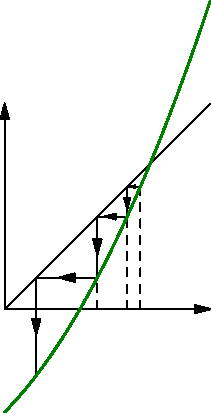
\includegraphics{C4792_1.pdf}
 % C4792_1.pdf: 99x198 pixel, 72dpi, 3.49x6.99 cm, bb=0 0 99 198
 \caption{Divergence monotone}
 \label{fig:C4792_1}
\end{figure}

\begin{prop}
 Lorsque $I$ est un intervalle stable pour $f$ et que $f$ est croissante sur $I$, alors, pour toute condition initiale $x_0\in I$, la suite $(x_n)_{n\in \N}$ est monotone.
\end{prop}
\begin{demo}
 En fait la première inégalité, celle entre les valeurs $x_0$ et $x_1$, va \emph{se propager} par récurrence:
\begin{align*}
 x_0\leq x_1 &\Rightarrow \forall n \in \N : x_n \leq x_{n+1} &:\text{ suite croissante}\\
x_0\geq x_1 &\Rightarrow \forall n \in \N : x_n \geq x_{n+1} &:\text{ suite décroissante}
\end{align*}
\end{demo}

\subsubsection{Fonction décroissante}
Soit $I$ un intervalle stable par une fonction $f$. Si $f$ est décroissante dans $I$ alors $f\circ f$ est croissante. Les suite \emph{extraites} d'indices pairs ou impairs sont monotones. On obtient des figures présentant des \og escargots\fg~ convergents ou divergents.

\subsubsection{Conditions suffisantes de stabilité ou d'instabilité}
Lorsque le signe de $f(x)-x$ est connu dans un intervalle autour d'un point fixe, on peut parfois savoir si ce point est stable ou instable.
\begin{itemize}
 \item Le point fixe est \emph{instable} lorsque la distribution des signes dans un intervalle $J$ est comme dans le tableau suivant :
\begin{center}
\renewcommand{\arraystretch}{1.5}
 \begin{tabular}{|c|ccc|}\hline
   &  & a &  \\  \hline
 f(x)-x   & - & 0 & + \\ \hline
\end{tabular}
\end{center}\bigskip
Lorsque la fonction est $\mathcal C^1$ dans $J$, la condition $f'(a)>1$ entraine une telle distribution locale des signes.

 \item Le point fixe est \emph{stable} lorsque la distribution des signes dans un intervalle $J$ est comme dans le tableau suivant :
\begin{center}
\renewcommand{\arraystretch}{1.5}
 \begin{tabular}{|c|ccc|}\hline
   &  & a &  \\  \hline
 f(x)-x   & + & 0 & - \\ \hline
\end{tabular}
\end{center}\bigskip
Lorsque la fonction est $\mathcal C^1$ dans $J$, la condition $0\leq f'(a) < 1$ entraine une telle distribution locale des signes.
\end{itemize}

\section{Fonctions à valeurs complexes}
dérivabilité par développement, caractérisation par partie réelle et imaginaire.\newline
Attention pas de théorème des accroissements finis, seulement l'inégalité des accroissements finis.

à compléter

\end{document}
